In this chapter, we present phenomenological
results for the production of a weak vector boson $V$ in association
with up to 5 jets for $V=W^+$ and $W^-$, and with up to 4 jets for
$V=Z$ at the LHC $\sqrt{s} = 13$ TeV, as shown in Ref.~\cite{Anger:2017nkq}. We
first present our results for total cross sections and differential
distributions and then for a series of observable ratios. In
particular, we explore uncertainties associated to renormalization
and factorization scales by using different functional forms for the
dynamical scales, as laid out in Section~\ref{sec_scales}. In general the structure of QCD corrections is very similar for the
different vector bosons $W^\pm$ and $Z$ and we often show results only for one type of weak vector boson.

\section{Total Cross Sections}
\label{totalxsv}
We quote total cross sections in Tables~\ref{tab_Wpj_total_xsv}, \ref{tab_Wmj_total_xs}
and~\ref{tab_Zj_total_xs} for the production of
a weak vector boson $V$ in association with up to 5 jets for $V=W^+$ and $W^-$,
and with up to 4 jets for $V=Z$, respectively. We include
results obtained with a central scale
$\HTpartonicp/2$ as well as those obtained with \MINLOp{} (see
section~\ref{sec_scale_notation} for the nomenclature that we use for the
different dynamical scales considered). Furthermore, in
Table~\ref{tab_jet_prod_total_xs} we show jet production
ratios~\cite{JetRatios1,JetRatios2,JetRatios3,JetRatios4,BH:Wratios}
for all vector boson types, that is ratios of total cross sections for the production for $V+n$ jets to the
production of $V+(n-1)$ jets.

%%%%%%%%%%% TABLE xs1 Wpnj-13TeV antikt %%%%%%%%%%%%%%%%%%%%%%%%%%
\begin{table}[p]
  \setlength{\tabcolsep}{1.6pt}
  \small
  \begin{tabular}{@{} c
      @{\hspace*{\lengthd}}     c
      @{\hspace*{\lengthd}}c
      @{\hspace*{\lengthc}}c
      @{\hspace*{\lengthc}}c
      @{\hspace*{\lengthd}}c
      @{\hspace*{\lengthd}}c @{}}
    \hline\hline
    \noalign{\vskip 2.5mm}
      jets  & $W^+$ LO & $W^+$ NLO & $W^+$ \MILOp{} & $W^+$ \MINLOp{} & \MILOp{}/LO &  \MINLOp{}/NLO\\
    \noalign{\vskip 2mm}
    \hline
    \noalign{\vskip 2mm}
      1 & $588.49(33)^{+23.77}_{-27.07}$ & $764.9(16)^{+37.8}_{-27.1}$
      & $591.50(35)^{+20.70}_{-25.36}$ & $799.1(18)^{+49.9}_{-35.1}$ &
      $1.005(1)$ & $1.045(3)$ \\
    \noalign{\vskip 2mm}
      2 & $197.23(27)^{+44.64}_{-34.42}$ &
      $197.78(66)^{+1.80}_{-7.82}$ &$205.01(28)^{+46.95}_{-36.46}$ &
      $211.44(78)^{+9.50}_{-12.07}$ & $1.039(2)$ & $1.069(5)$ \\
    \noalign{\vskip 2mm}
      3 & $57.07(10)^{+22.82}_{-15.23}$ & $49.54(27)^{+0.00}_{-3.13}$ &
      $59.09(11)^{+26.02}_{-16.89}$ & $52.32(41)^{+0.19}_{-3.95}$ & $1.035(3)$
      & $1.056(10)$\\
    \noalign{\vskip 2mm}
      4 & $16.408(50)^{+9.344}_{-5.566}$ & $12.14(22)^{+0.00}_{-1.59}$ &
      $17.287(56)^{+11.768}_{-6.516}$ & $12.78(24)^{+0.00}_{-2.87}$
      &$1.054(5)$ & $1.053(27)$\\
    \noalign{\vskip 2mm}
      5 & $4.579(45)^{+3.399}_{-1.829}$ & $3.06(14)^{+0.00}_{-0.72}$ &
      $4.908(56)^{+4.691}_{-2.233}$ & $3.21(14)^{+0.00}_{-0.52}$ &
      $1.072(16)$ & $1.049(66)$ \\
    \noalign{\vskip 2mm}    
    \hline\hline
    \end{tabular}
\caption{LO and NLO QCD results for inclusive $W^++1,2,3,4,5$-jet total cross sections
(in $pb$). We quote results for the two dynamical scales, $\HTpartonicp/2$ and
\MINLOp{}, as well as their ratios. Details of the setup are given in section~\ref{sec_kin}.
We determine the conventional scale dependence by varying both $\mu_R$
and $\mu_F$ by factors of $2$ and $\sqrt{2}$ up and down. The
statistical integration error is given in parenthesis. \label{tab_Wpj_total_xsv} }
\end{table}

%%%%%%%%%%% TABLE xs1 Wmnj-13TeV antikt %%%%%%%%%%%%%%%%%%%%%%%%%%
\begin{table}[p]
  \setlength{\tabcolsep}{1.6pt}
  \small
  \begin{tabular}{@{} c
      @{\hspace*{\lengthd}}     c
      @{\hspace*{\lengthd}}c
      @{\hspace*{\lengthc}}c
      @{\hspace*{\lengthc}}c
      @{\hspace*{\lengthd}}c
      @{\hspace*{\lengthd}}c @{}}
    \hline\hline
    \noalign{\vskip 2.5mm}
      jets  & $W^-$ LO & $W^-$ NLO & $W^-$ \MILOp{} & $W^-$ \MINLOp{} &\MILOp{}/LO &\MINLOp{}/NLO \\
      \noalign{\vskip 2mm}
      \hline
      \noalign{\vskip 2mm}
      1 & $446.68(22)^{+17.48}_{-20.29}$ & $582.0(11)^{+25.6}_{-18.6}$
      &  $448.82(23)^{+15.07}_{-18.92}$ & $608.2(12)^{+34.6}_{-24.5}$
      & $1.005(1)$ & $1.045(3)$ \\
    \noalign{\vskip 2mm}
      2 & $141.67(14)^{+31.89}_{-24.67}$ &
      $144.53(39)^{+1.03}_{-5.46}$ & $147.40(15)^{+33.40}_{-26.08}$ &
      $154.11(46)^{+5.91}_{-8.40}$& $1.040(1)$ & $1.066(4)$ \\
    \noalign{\vskip 2mm}
      3 & $39.029(55)^{+15.653}_{-10.448}$ &
      $34.34(16)^{+0.00}_{-2.10}$ & $40.889(61)^{+17.99}_{-11.70}$ &
      $36.20(22)^{+0.03}_{-2.64}$ & $1.048(2)$ & $1.054(8)$\\
    \noalign{\vskip 2mm}
      4 & $10.513(23)^{+6.035}_{-3.585}$ & $8.22(13)^{+0.00}_{-0.86}$
      & $11.399(27)^{+7.797}_{-4.314}$ & $8.85(19)^{+0.00}_{-1.85}$ &
      $1.084(3)$ & $1.077(29)$ \\
    \noalign{\vskip 2mm}
      5 & $2.747(12)^{+2.059}_{-1.103}$ &
      $1.971(56)^{+0.004}_{-0.298}$ & $3.063(14)^{+2.949}_{-1.400}$ &
      $2.105(59)^{+0.000}_{-0.788}$ &$1.115(7)$ & $1.068(43)$\\
    \noalign{\vskip 2mm}    
    \hline\hline
    \end{tabular}
\caption{As in Table~\ref{tab_Wpj_total_xsv} but for inclusive
  $W^-+1,2,3,4,5$-jet total cross sections.\label{tab_Wmj_total_xs} }
\end{table}

%%%%%%%%%%% TABLE xs1 Znj-13TeV antikt %%%%%%%%%%%%%%%%%%%%%%%%%%
\begin{table}[p]
  \setlength{\tabcolsep}{1.6pt}
  \footnotesize 
  \begin{tabular}{@{} c
      @{\hspace*{\lengthd}}     c
      @{\hspace*{\lengthd}}c
      @{\hspace*{\lengthc}}c
      @{\hspace*{\lengthc}}c
      @{\hspace*{\lengthd}}c
      @{\hspace*{\lengthd}}c @{}}
    \hline\hline
    \noalign{\vskip 2.5mm}
      jets  & $Z$ LO & $Z$ NLO  & $Z$ \MILOp{} & $Z$ \MINLOp{} & \MILOp{}/LO & \MINLOp{}/NLO  \\
      \noalign{\vskip 2mm}
      \hline
      \noalign{\vskip 2mm}
      1 & $112.264(60)^{+4.121}_{-4.876}$ &
      $142.79(15)^{+5.12}_{-3.70}$ & $112.615(43)^{+3.390}_{-4.448}$ &
      $148.48(17)^{+7.21}_{-5.04}$ & $1.003(1)$ & $1.040(2)$\\
    \noalign{\vskip 2mm}
      2 & $36.140(38)^{+7.931}_{-6.178}$ &
      $36.811(65)^{+0.228}_{-1.339}$ & $36.780(28)^{+8.076}_{-6.382}$
      & $38.962(68)^{+1.555}_{-2.147}$ & $1.018(1)$ & $1.058(3)$\\
    \noalign{\vskip 2mm}
      3 & $10.4844(76)^{+4.1227}_{-2.7702}$ & $9.175(44)^{+0.000}_{-0.578}$
      &  $11.1242(87)^{+4.847}_{-3.166}$ & $9.612(50)^{+0.000}_{-0.617}$ &
      $1.061(1)$ & $1.048(7)$\\
    \noalign{\vskip 2mm}
      4 & $2.9597(37)^{+1.6698}_{-0.9989}$ &
      $2.331(29)^{+0.000}_{-0.246}$ & $3.3050(43)^{+2.248}_{-1.247}$ &
      $2.439(37)^{+0.000}_{-0.668}$ & $1.117(2)$ & $1.046(21)$\\
    \noalign{\vskip 2mm}    
    \hline\hline
    \end{tabular}
\caption{As in Table~\ref{tab_Wpj_total_xsv} but for inclusive
  $Z+1,2,3,4$-jet total cross sections.\label{tab_Zj_total_xs} }
\end{table}



%scale dependence for Wm
%%%%%%%%%%%%% FIGURE %%%%%%%%%%%%%%%%%%
\begin{figure}[p]
\begin{center}
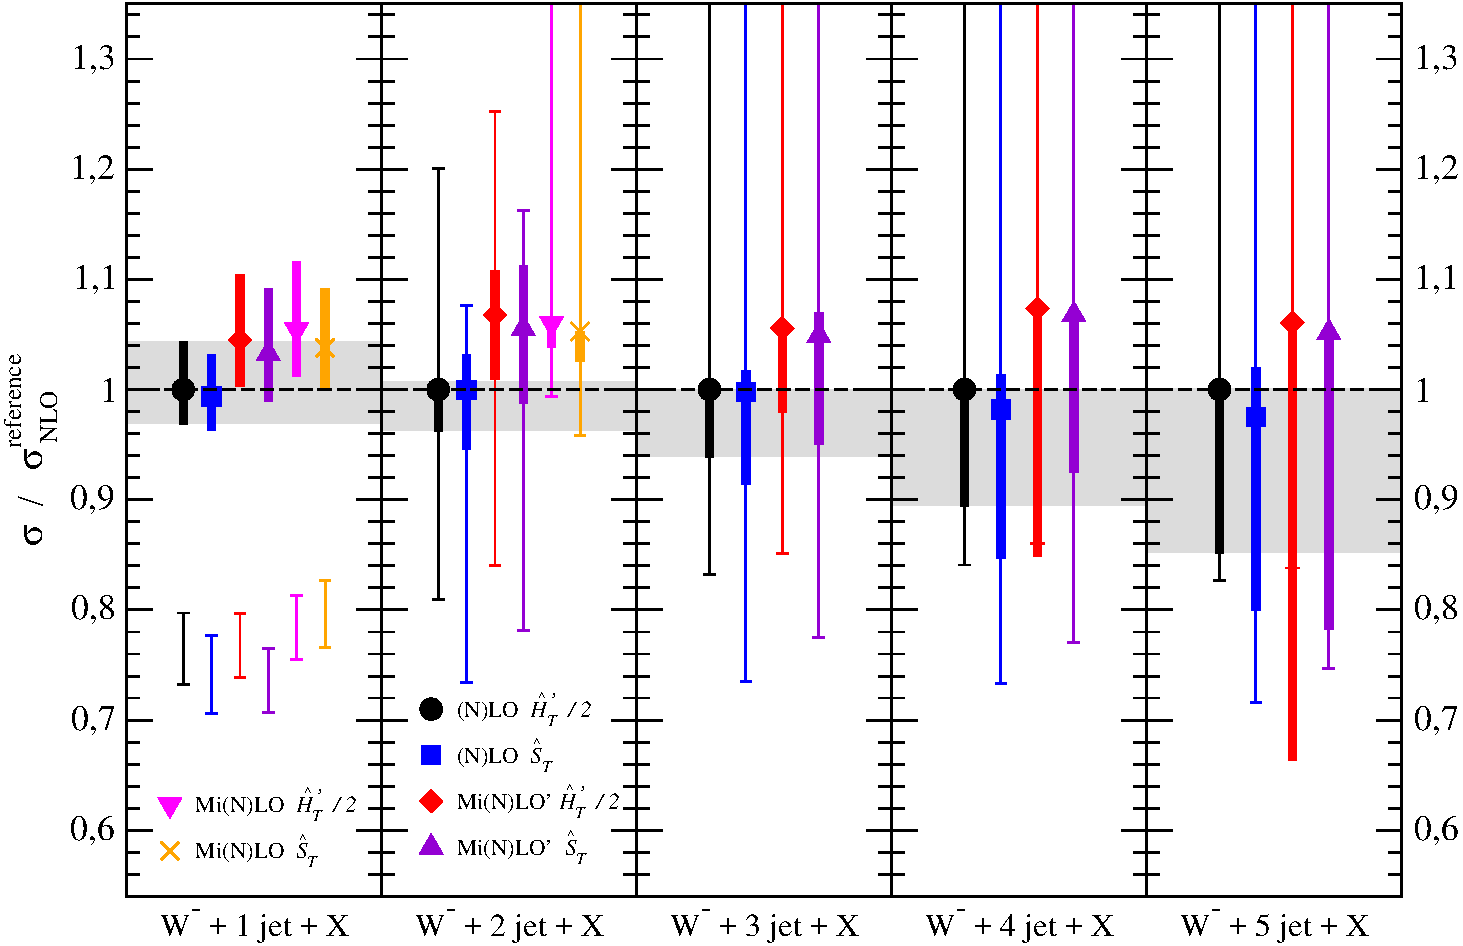
\includegraphics[clip,scale=0.65]{plots/multi_scales_Wm}
\end{center}
\caption{Scale dependence of total cross sections for inclusive
$W^-+1,2,3,4,5$-jet production considering all scales defined in
section~\ref{sec_scale_notation} for both LO and NLO results. The corresponding symbols and colors are specified in the legend of the plot. The LO scale-dependence bands are represented by thin lines (in certain cases extending outside of
the range plotted) while the thick lines represent NLO bands. We
normalized all
results to the corresponding NLO $\HTpartonicp/2$ result for each jet
multiplicity and the gray bands show the NLO $\HTpartonicp/2$ scale-dependence band.}
\label{fig_Wp_all_scales}
\end{figure}
%%%%%%%%%%%%%%%%%%%%%%%%%%%%%%%%%%%%%%%



%%%%%%%%%%% TABLE xs1 jet_production_ratios_13TeV
%%%%%%%%%%% antikt %%%%%%%%%%%%%%%%%%%%%%%%%%
\begin{table}[]
  \small
        \begin{tabular}{@{} c
            @{\hspace*{\lengthe}}c
            @{\hspace*{\lengthe}}c
            @{\hspace*{\lengthe}}c
            @{\hspace*{\lengthe}}c
            @{\hspace*{\lengthe}}c
            @{\hspace*{\lengthe}}c
            @{\hspace*{\lengthe}}c
            @{\hspace*{\lengthe}}c
            @{\hspace*{\lengthe}}c @{}}
          \hline\hline
          \noalign{\vskip 2.5mm}
        \multicolumn{1}{c}{ } & \multicolumn{3}{c}{$W^+ n/(n-1)$} &
        \multicolumn{3}{c}{$W^- n/(n-1)$}  & \multicolumn{3}{c}{$Z n/(n-1)$} \\
        \noalign{\vskip 2mm}
        \hline
        \noalign{\vskip 2mm}
        $n$ & LO & NLO & \MINLOp{} & LO & NLO & \MINLOp{}
        & LO & NLO & \MINLOp{} \\
        \noalign{\vskip 2mm}
        \hline
        \noalign{\vskip 2mm}
        2 &  $0.3351(5)$ & $0.259(1)$ & $0.265(1)$ &$0.3172(4)$ &
        $0.248(1)$ &$0.253(1)$& $0.3219(4) $ & $0.2578(5)$
        &$0.2624(5)$ \\
  \noalign{\vskip 2mm}
        3 &  $0.2894(6)$ & $0.250(2)$ &$0.247(2)$ &$0.2755(5)$ &
        $0.238(1)$ &$0.235(2)$& $0.2901(4)$ & $0.249(1)$&$0.247(1)$\\
  \noalign{\vskip 2mm}
        4 &  $0.288(1)$ & $0.245(5)$ &$0.244(5)$ &$0.2694(7)$ &
        $0.239(4)$ &$0.244(5)$& $0.2823(4)$ & $0.254(3)$&$0.254(4)$\\
  \noalign{\vskip 2mm}
        5 &  $0.279(3)$ & $0.252(12)$ &$0.251(11)$ &  $0.261(1)$ & $0.240(8)$ &$0.238(8)$& ---
        & --- & ---\\
    \noalign{\vskip 2mm}    
    \hline\hline   
      \end{tabular}
\caption{LO, NLO and \MINLOp{} QCD jet production ratios for $W^{\pm}$ as well as
$Z/\gamma^*$. The ratio is taken for a given process to that with one fewer jet.
The setup is specified in section~\ref{sec_kin}. The
number in parenthesis next to the ratio gives the corresponding statistical
integration error.\label{tab_jet_prod_total_xs} }
\end{table}

The scale dependence of LO cross sections for the scale choice
$\mu_0=\HTpartonicp/2$ is monotonically increasing with jet multiplicity. The
LO scale dependence for $V+1$ jet, which appears at around 4\% is not
representative of the associated theoretical uncertainties, in particular due to
kinematical constraints that are released at NLO. In this situation, at LO the $p_{\textrm T}$
of the vector boson matches the one from the unique jet. Real contributions at
NLO release this constraint, producing a soft enhancement that tends to produce
large corrections~\cite{Bauer:2009km,BH:W3jDistributions,Rubin:2010xp}. The total cross section at the central scale choice for the dynamical scale $\mu_0=\HTpartonicp/2$
lies near the plateau of the NLO scale dependence. Resultingly, the
uncertainty estimates based on lower/upper values of the cross sections seem slightly
small. If we quote the absolute deviations with respect to this value, we
can estimate NLO scale sensitivity at the order of 10\% (running from about 6\%
to 16\%, depending on multiplicity). 

The total cross sections with \MILOp{} are similar to the corresponding LO
results. However, the absolute predictions tend to be larger for
\MILOp{} with the excess increasing slightly with multiplicity. The
central prediction of the \MINLOp{} results agree
well with the NLO results. Moreover, their ratio is relatively stable as a function of jet multiplicity.


We display total cross sections and the corresponding scale variations for $W^-$ production in association with jets for all scales considered in this analysis in
Fig.~\ref{fig_Wp_all_scales}. We observe that in particular the \MILOp{} and \MINLOp{} predictions
exhibit a considerable variation for different choices of $\mu_{\textrm core}$, both in their central value and in
the associated conventional scale uncertainty. The sensitivity on the core scale can be traced to the procedure for the identification of ordered clustering
hierarchies (cf. Sec.~\ref{sec_minlo_gen}). The clustering is terminated as soon as an inverted scale hierarchy is encountered and the remaining ``core'' process as evaluated at $\mu_{\textrm core}$. For events with many hard scales, this biases the scale choice towards $\mu_{\textrm core}$,
and therefore the precise definition of $\mu_{\textrm core}$ plays a
significant role~\cite{CKKWincl}. On average, the choice of
$\HTpartonicpp$ increases $\mu_{\textrm core}$ and thus permits more clusterings in high-multiplicity final states and therefore induces more associated
Sudakov form factors. Resultingly, both central value of the prediction
and the related scale uncertainty are reduced on average.

In Table~\ref{tab_jet_prod_total_xs} we show jet-production ratios. In these ratios many uncertainties associated to scale sensitivity and
PDF dependence cancel. Also systematic
uncertainties in experimental analyses associated with luminosity
measurements cancel. Overall, we observe a remarkable stability of these
ratios at NLO for both scale choices $\HTpartonicp/2$ and \MINLOp{},
with the ratio for all of them being around a value of $0.25$. This universality
is present for NLO ratios in $V+$jet production even though the
corresponding LO ratios deviate considerably. One can use this
universality of the jet production ratios for tests of the SM and they
can be exploited to make extrapolations of
total and differential cross sections to larger jet-multiplicity
processes~\cite{BH:Wratios}.


%scale dependence for Wm
%%%%%%%%%%%%% FIGURE %%%%%%%%%%%%%%%%%%
\begin{figure}[t]
\begin{center}
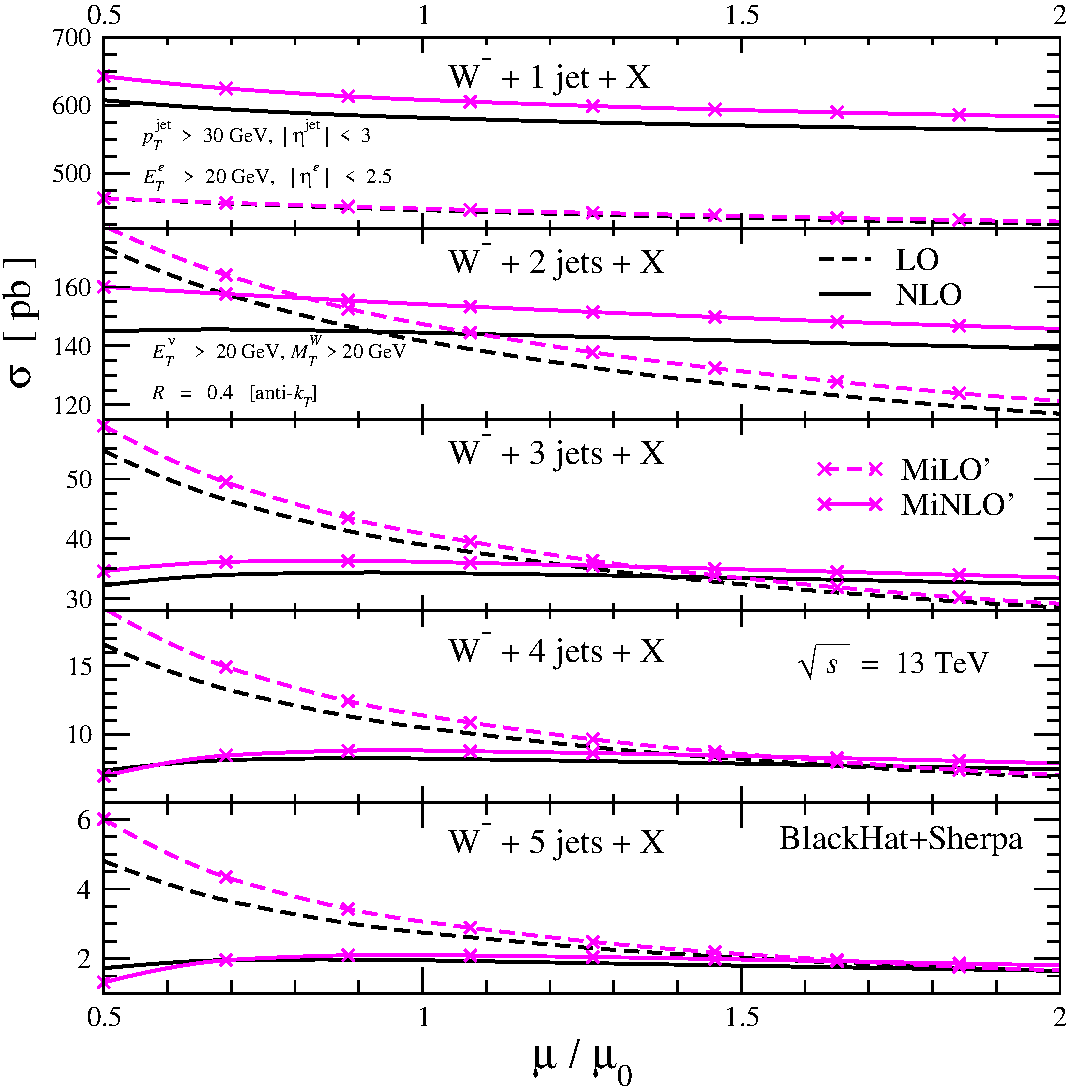
\includegraphics[clip,scale=0.75]{plots/Wmnj-13TeV_dyn_scale_dependence}
\end{center}
\caption{Renormalization- and factorization-scale dependence of total cross
  sections for inclusive $W^-+1,2,3,4,5$-jet production. For each
  multiplicity, we show the dependence of predictions at LO as dashed (black) lines
  and at NLO as solid (black) lines with $\mu_0=\mu_{\textrm r}=\mu_{\textrm f}=\HTpartonicp/2$, while predictions for \MILOp{}
  are shown as dashed-crossed (magenta) lines and those for \MINLOp{} as solid-crossed (magenta) lines.}
\label{fig_Wmjets_sdep}
\end{figure}
%%%%%%%%%%%%%%%%%%%%%%%%%%%%%%%%%%%%%%%


\section{Scale Dependence}\label{vscale}
In Fig.~\ref{fig_Wmjets_sdep} we display the dependence of total cross sections
in $W^-$ production in association with up to 5 jets on renormalization
and factorization scales. Both LO and \MILOp{} results are very sensitive
to these scales. However, we find a remarkable stability for both NLO
and \MINLOp{} results, with the central prediction lying at the plateau of the NLO curves for
$W^-+$3,4 and 5 jets, thus minimizing the scale variations (for a discussion of this effect, see~\cite{BH:W3jDistributions}).


The LO results obtained with the two scale choices are largely consistent in both normalization and scale sensitivity since the difference between the results is smaller than the respective factor-two scale variations. \MILOp{}
results are slightly larger compared to the LO results obtained with $\HTpartonicp/2$.
%
We attribute this to the fact that the smaller average renormalization scales
for large jet multiplicity in \MILOp{} and the correspondingly large strong couplings
are not entirely compensated by the suppression from Sudakov form
factors. We also note that the two LO results differ slightly in their
variation. Whereas the scale uncertainty at low multiplicity
associated to LO and \MILOp{} results are comparable, the \MILOp{}
results exhibit larger scale variations with increased
multiplicity.


The NLO results obtained with both dynamical scales are mostly
consistent. For the case of multiplicities with more than $2$ jets, the differences between
the two scale choices lie within the respective factor-two scale
variations. For the case of $W+2$-jet production, we observe an
approximately 15\% discrepancy which can be taken as an estimate for the total scale uncertainty
associated with this prediction. We furthermore observe that with increasing
multiplicity, the bands associated to the uncertainty of the respective scale
choice seem to behave differently between $\HTpartonicp/2$ and the \MINLOp{}
scheme. In general, the scale uncertainty obtained by factor-two variations
grows with multiplicity, a trend that is slightly more pronounced for the
\MINLOp{} scale choice.

%pt of four softest jets
%%%%%%%%%%%%% FIGURE %%%%%%%%%%%%%%%%%%
\begin{figure}[t]

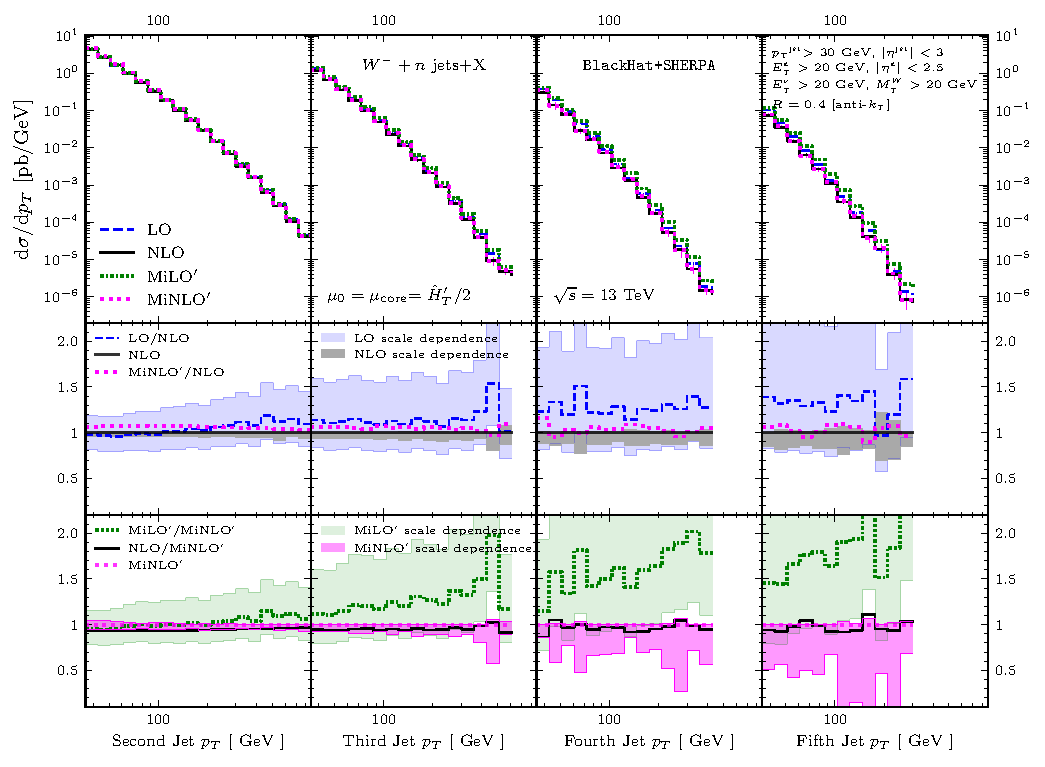
\includegraphics[clip,scale=0.95]{plots/Wmnj-13TeV_anti-kt-R4-Pt30_jets_jet_1_1_pt__Kn}
\caption{The $\pT$ spectra of the softest jet (ordered in $p_T$) in inclusive
  samples of $W^-+n$ jets ($n=2,3,4,5$) at the LHC at $\sqrt{s}=13$~TeV. In the upper panels, we show NLO predictions as solid (black) lines, \MINLOp{} predictions as dotted
(magenta) lines, while LO predictions are shown as dashed (blue) lines
and \MILOp{} predictions as dash-dotted (green) lines. In the
central panels, we show predictions for both LO and \MINLOp{} distribution as
well as scale-dependence bands at NLO (grey) and LO (blue) normalized to the central NLO
prediction. Similarly in the bottom panels, we show predictions for \MILOp{} and NLO distributions as well
as scale dependence bands for
\MILOp{} (green) and
\MINLOp{} (magenta) normalized to the central \MINLOp{} predictions.}
\label{fig_Wmnjptv}
\end{figure}
%%%%%%%%%%%%%%%%%%%%%%%%%%%%%

%HT distribution
%%%%%%%%%%%%% FIGURE %%%%%%%%%%%%%%%%%%
\begin{figure}[t]

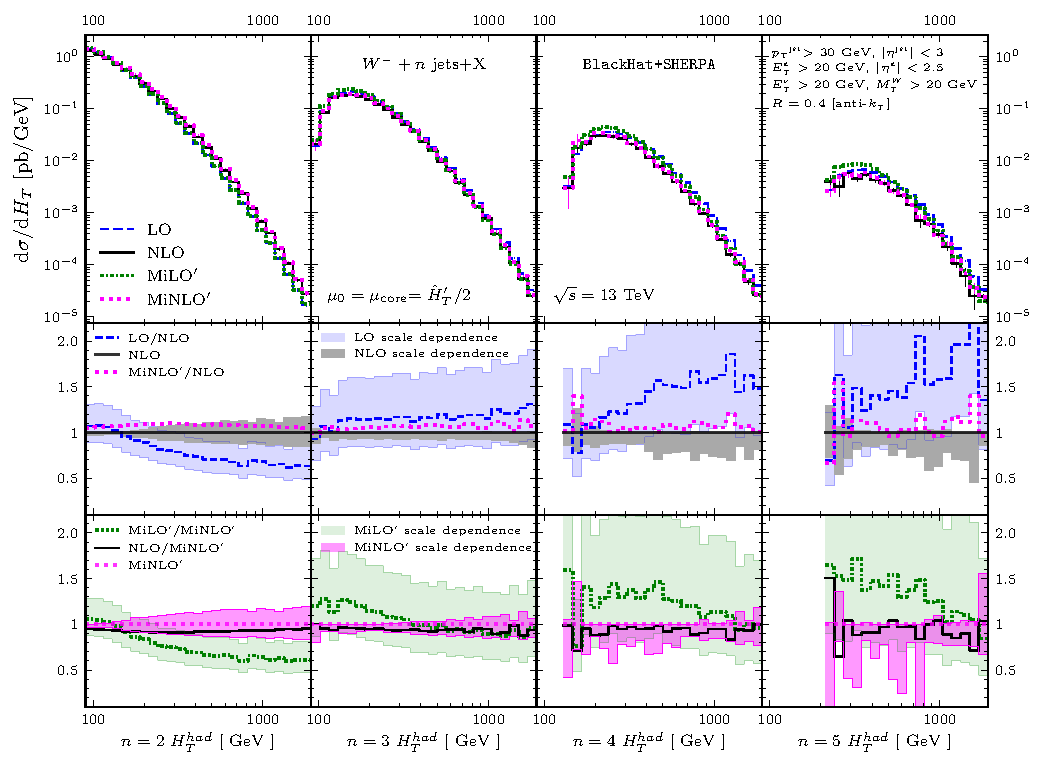
\includegraphics[clip,scale=0.95]{plots/Wmnj-13TeV_anti-kt-R4-Pt30_jets_HT_C}
\caption{Distribution in the total hadronic transverse energy $H_T^{had}$ in inclusive samples
of $W^-+2,3,4,5$-jets. Format as in Figure~\ref{fig_Wmnjptv}.
}
\label{fig_Wmjets_HT}
\end{figure}
%%%%%%%%%%%%%%%%%%%%%%%%%%%%%

%HT distribution
%%%%%%%%%%%%% FIGURE %%%%%%%%%%%%%%%%%%
\begin{figure}[t]

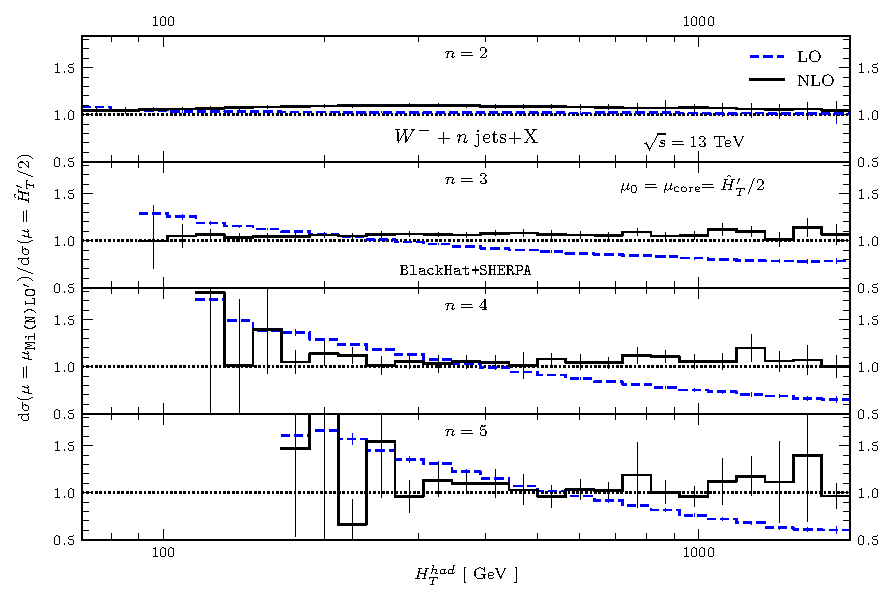
\includegraphics[clip,scale=1]{plots/rat_Wmnj_MINLO_HT_anti-kt-R4-Pt30_jets_HT_C}
\caption{Ratio of the distribution in the total hadronic transverse energy $H_{\textrm T}^{had}$ in inclusive samples of \Wmjn-jet production ($n=2,3,4$ and $5$) comparing the \MINLOp{} and $\HTpartonicp/2$ scale choice.}
\label{fig_MINLO_HTp_ratios_HT}
\end{figure}
%%%%%%%%%%%%%%%%%%%%%%%%%%%%%



\section{Differential Cross Sections}
\label{diffxswv}

In this section we present several differential cross sections and show
the impact that next-to-leading order corrections have on fixed-order predictions over
phase space. We show results only for the $W^-$ weak vector boson,
as in general the structure of QCD corrections is very similar for the
different vector bosons $W^\pm$ and $Z$. We include (N)LO and \MILNLOp{} results and do not show results for the scale choice $\HTpartonicpp$, since they are rather consistent with the ones obtained with $\HTpartonic/2$.



In Fig.~\ref{fig_Wmnjptv} we show $p_T$ spectra of the softest jet (ordered in $p_T$) for the production of $W^-$+$n$ jets with $n$ ranging from $n=2$ to $n=5$. Solid (black) lines show NLO predictions, dotted (magenta) lines
\MINLOp{} predictions, while dashed (blue) lines show LO predictions
and dash-dotted lines \MILOp{} predictions. The thin vertical lines
represent the estimate of statistical integration errors. In the middle panels, we show ratios of LO, NLO and \MINLOp{} to the NLO result including scale
dependence bands at LO (blue) and NLO (grey). Similarly, the lower panels show
ratios of \MILOp{}, NLO and \MINLOp{} to the \MINLOp{} results and
scale dependences for \MILOp{} (green) and
\MINLOp{} (magenta). Previous studies at lower energies (see for example~\cite{BH:W5j}) have
shown that the $n$-th jet $p_{\textrm T}$ spectrum in an inclusive $V+n$ jets sample
tends to have rather small distortions due to QCD corrections (as long
as $n>1$). We can confirm this result with our current study, with the
LO to NLO ratios being flat over a wide $p_T$ range. It is clear that
although LO results employing an $\HTpartonicp/2$ dynamical scale have similar shapes to the NLO results, their
normalization is badly determined, following the trend described in the
previous section on total cross sections. Furthermore, we notice that \MINLOp{}
results are in good agreement with NLO results regarding both shape and
normalization over the seven orders of magnitude shown for the differential
cross sections. Using the $\HTpartonicp/2$ scale-dependence
band as well as its deviation with respect to the \MINLOp{} result as a measure of the associated uncertainties, we can confirm the relatively good theoretical control over NLO prediction for these observables and estimate related uncertainties to the order of 15\%.



In Fig.~\ref{fig_Wmjets_HT} we study the differential distribution in
the total hadronic transverse energy $H_{\textrm T}^{had}$ as well as ratios thereof
between \MILNLOp{} and $\HTpartonicp/2$ scale choices in
Fig.~\ref{fig_MINLO_HTp_ratios_HT}. The format of Fig.~\ref{fig_Wmjets_HT} is as
in Fig.~\ref{fig_Wmnjptv}, that is we show in side-by-side panels results for $W^-+n$
jets, with $n=2$, $3$, $4$ and $5$. For $n\ge 3$, we find that the corrections to the $H_{\textrm T}^{had}$ spectrum change the shape of the
distributions relatively mild in general, which can be seen by looking at both LO to NLO ratios as well
as \MINLOp{} to NLO ratios. Notice that the fluctuations at NLO for small
values of $H_{\textrm T}^{had}$ for increasing multiplicity are just due to the fact
that near threshold the integration errors grow large. On the other hand, the
$n=2$ LO predictions have a large shape difference compared to the NLO
results. These changes are similar to the corresponding observable for $n=1$ for which it is well
known that large corrections appear from configurations with many jets in the
final state~\cite{Rubin:2010xp}. The widening of the NLO scale band indeed shows that real
contributions are large in the tail of the distributions, making this observable
sensitive to quantum corrections. In principle a computation of NNLO QCD correction to $V+2$
jets would be desirable in order to stabilize the predictions.

We notice an interesting behavior in the ratios of $H_{\textrm T}^{had}$ distributions between \MILNLOp{} and $\HTpartonicp/2$ scale choices as shown in Fig.~\ref{fig_MINLO_HTp_ratios_HT}. At NLO, these ratios are quite stable and lie around 1. For the $n=2$ case, the ratio between \MILOp{} and LO results is also stable and lies around 1. However, for the higher multiplicity cases the LO ratios become tilted with a negative slope. This trend becomes more pronounced with light-jet multiplicity. We attribute this to the fact that very
large values of $H_{\textrm T}^{had}$ are mostly generated in events of di-jet type with largely
disparate scales of jet production, i.e.\ $p_{T,j1}\approx p_{T,j1}\gg p_{T,j3},\ldots,p_{T,jn}$. In the \MILOp{} method, this induces Sudakov suppression factors that reduce the corresponding high-$H_{\textrm T}^{had}$
tails compared to the LO prediction. However, these factors improve the agreement of \MILOp{} with the \MINLOp{} prediction as visible in the bottom panels of Fig.~\ref{fig_Wmjets_HT}.

%pt of four softest jets
%%%%%%%%%%%%% FIGURE %%%%%%%%%%%%%%%%%%
\begin{figure}[t]
  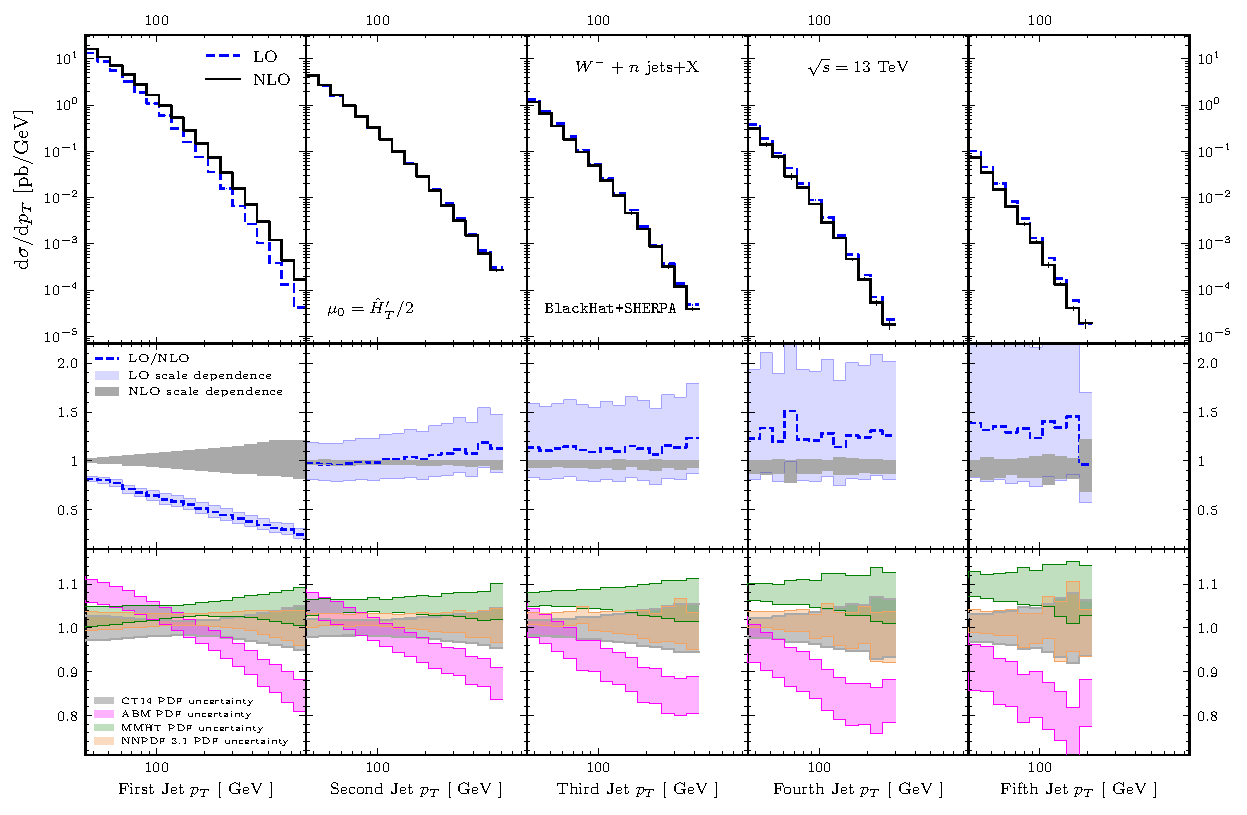
\includegraphics[clip,scale=0.80]{plots/Wmnj-13TeV_anti-kt-R4-Pt30_jets_jet_1_1_pt__Kn_PDF}
\caption{PDF uncertainty for the $\pT$ distribution of the softest jet in an inclusive sample
of $W^-+n$ jets ($n=1,2,3,4,5$) at the LHC at $\sqrt{s}=13$~TeV. In the
  upper panels, we show NLO predictions as solid (black) lines and LO predictions as dashed (blue) lines. The
central panels show the scale-dependence bands at NLO (grey) and LO
(blue) normalized to the central NLO prediction. The lower
panels show the NLO PDF uncertainty for CT14 (gray), ABM
(magenta), MMHT (green) and NNPDF 3.1 (orange) PDF
sets, normalized to the results obtained with CT14.}
\label{fig_WmnjptPDF}
\end{figure}

%%%%%%%%%%% TABLE central PDF vals %%%%%%%%%%%%%%%%%%%%%%%%%%
\begin{table}
\begin{center}
    \begin{tabular}{cccccc}
        \hline\hline
        \noalign{\vskip 2.5mm}
      nbr. of jets  &  1&	2&	3&	4&	5\\
      \noalign{\vskip 2mm}
      \hline
      \noalign{\vskip 2mm}
      CT14      &$1.000$  &$1.000$  &$1.000$  &$1.000$   &$1.000$  \\
     \noalign{\vskip 2mm}
      ABM       &$1.070$ &$1.039$  &$1.000$ &$0.960$  &$0.920$ \\     \noalign{\vskip 2mm}
      MMHT      &$1.029$ &$1.049$  &$1.066$ &$1.080$  &$1.095$ \\     \noalign{\vskip 2mm}
      NNPDF 3.1 &$1.016$ &$1.018$  &$1.020$ &$1.020$  &$1.016$  \\
      \noalign{\vskip 2mm}
\hline\hline
    \end{tabular}
\end{center}
\caption{NLO QCD total cross sections for inclusive
$W^-+1,2,3,4,5$-jet production for different choices of PDF sets, normalized to the
results for CT14. This data was generated by creating a fastNLO
table \cite{Britzger:2012bs} from the \ntuple{} data.}
\label{tab_Wmj_pdf_central}
\end{table}


In Figure~\ref{fig_WmnjptPDF} we explore uncertainties associated to
the choice of PDFs and show the PDF uncertainty bands for $n$th-jet $p_{\textrm T}$ spectra
in an inclusive sample of $W^-+$jets for $\HTpartonicp/2$, analogous to the distributions shown in
Fig.~\ref{fig_Wmnjptv}. The additional bottom panel shows the NLO PDF uncertainty
bands for CT14 (gray)~\cite{CT14}, ABM (magenta)~\cite{ABM}, MMHT
(green)~\cite{MMHT} and
NNPDF 3.1 (orange)~\cite{NNPDF} PDF
sets, all normalized to the central value obtained with CT14. 
We generated the data for Fig.~\ref{fig_WmnjptPDF} by
creating a fastNLO table~\cite{Britzger:2012bs} from our \ntuple{} data. We also quote the
central values for total cross sections obtained with the different
choices of PDF sets, normalized to the results for CT14, in Tab.~\ref{tab_Wmj_pdf_central}.


In our samples, PDF uncertainties can reach up to 10\% and most of the error sets
overlap. However, both central values and uncertainty bands of the ABM
results lie outside the uncertainty bands of all other PDF sets. Also, the MMHT bands
lie systematically higher than the others, a trend that is more pronounced in the
large-multiplicity cases. All uncertainty bands increase for larger
$p_{\textrm T}$ as the effective mass sampled for the corresponding
events grows and the PDFs are evaluated for larger values of the Bjorken $x$, with less data available to constrain the PDF
fits. PDF uncertainties are thus of the same order as NLO scale
uncertainties, in particular for the high-multiplicity processes,
where we observe a considerable spread between the different PDF sets. At the
level of normalized NLO QCD total cross sections this is shown in
Tab.~\ref{tab_Wmj_pdf_central}.


\section{Cross Section Ratios}
\label{sec_ratios}

In this
section, we study the differential jet ratio for $W^-$ production as
well as differential ratios of both $W^-/W^+$ and $Z/W$
production. These observable ratios feature reduced uncertainties compared to
basic observables such as cross sections or differential
distributions. In particular, experimental uncertainties related to jet energy
scale, lepton efficiency, acceptance and proton-proton luminosity should be
greatly reduced. Also the observable ratios are expected to suffer less from theoretical
uncertainties from uncalculated higher-order corrections. Furthermore, non-perturbative effects are expected to largely cancel in these observable ratios. When comparing parton-level result to experimental data, these non-perturbative effect such as hadronization of the outgoing partons or effects induced by the underlying event have to be accounted for. In consequence, these ratios can help to better understand the structure of quantum corrections to
processes with a vector boson in association with multiple jets and as shown
in~\cite{BH:Wratios} they exhibit certain universal features that
can be exploited in phenomenological studies at hadron colliders. 


% jet ratios for Wm production as function of the Wm PT and of HT
%%%%%%%%%%%%% FIGURE %%%%%%%%%%%%%%%%%%
\begin{figure}[t]

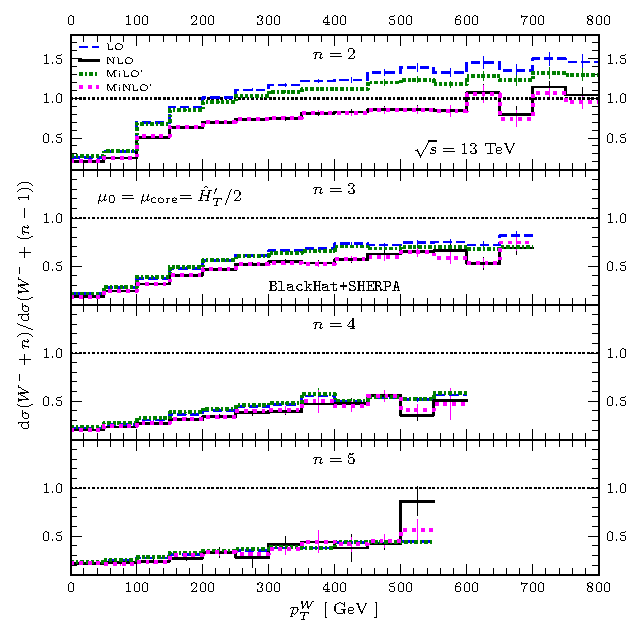
\includegraphics[clip,scale=0.75]{plots/jetratio_Wm_13TeV_anti-kt-R4-Pt30_PTe-veb_A}
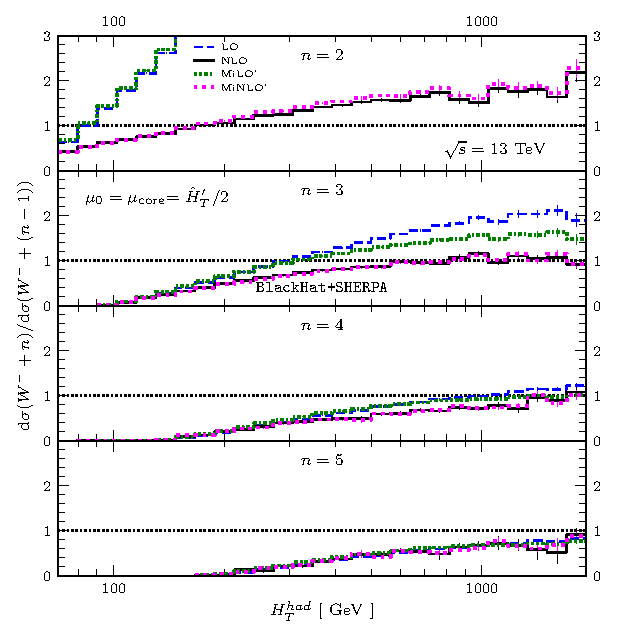
\includegraphics[clip,scale=0.75]{plots/jetratio_Wm_13TeV_anti-kt-R4-Pt30_jets_HT_C}
\caption{Ratios of \Wmjn-jet to \Wmjnm-jet cross sections as a function of
the transverse momentum $p_{\textrm T}^W$ of the $W^-$-boson on the left, and as a function of
the hadronic transverse energy $H_{\textrm T}^{had}$ on the right with $n=2$
(top panel) to $n=5$ (bottom panel). LO results are shown as dashed (blue) lines and NLO results as solid
(black) lines, while \MILOp{} results are shown as dash-dotted
(green) lines and \MINLOp{} results as dotted (magenta) lines.
}
\label{fig_jetrat}
\end{figure}
%%%%%%%%%%%%%%%%%%%%%%%%%%%%%

\subsection{Jet Ratios}
\label{sec_jetratio}

In Figure~\ref{fig_jetrat}, we show differential jet-production ratios of $W^-+n$-jet to $W^-+(n-1)$-jet production with up to $n=5$ jets as a function of the $W^-$-boson
transverse momentum $p_{\textrm T}^W$ in the left panel and of the total hadronic transverse energy $H_{\textrm
T}$ in the right panel. We show ratios for both scale choices with
$\HTpartonicp/2$ at LO shown as dashed (blue)
lines and at NLO as solid (black) lines, while \MILOp{} ratios are
shown as dash-dotted (green) lines and those for \MINLOp{} as
dotted (magenta) lines.



We observe that the \Wmjj-jet / \Wmj-jet ratio ($n=2$) as a function of $p_{\textrm T}^W$ shows large NLO corrections. This is mainly due to the large corrections
appearing at NLO~\cite{Rubin:2010xp}, which are related to the release of a kinematical constraint as described in the previous sections. The corresponding corrections at
NNLO~\cite{Boughezal:2015dva,Boughezal:2015ded,Gehrmann-DeRidder:2016zml}
are stabilized. In the lowest $p_{\textrm T}$ region (up to the order of the
$W$ mass), the ratios lie around a value of $0.25$, roughly independent of the
number of jets. In this region, the NLO corrections are modest for all
displayed multiplicities, which is in agreement with the total cross sections displayed in
Tab.~\ref{tab_Wmj_total_xs}. The ratios grow monotonically with $p_{\textrm T}^W$ and are stabilized for $n\geq 3$ for large $p_{\textrm T}^W$. The increase is
less pronounced for the higher-multiplicity cases and the ratio stabilizes for $n=5$ around a value
$0.5$. In the low-multiplicity cases ($n\leq 3$) and for large values of $p_{\textrm T}^W$, the ratio for
\MILOp{} lies below that for LO. The LO ratios in the higher-multiplicity
cases as well
as all those of NLO and \MINLOp{} agree very well. 
% charge asymmetry ratios for W production as function of the softest jets and  as function of HT
%%%%%%%%%%%%% FIGURE %%%%%%%%%%%%%%%%%%
\begin{figure}[t]

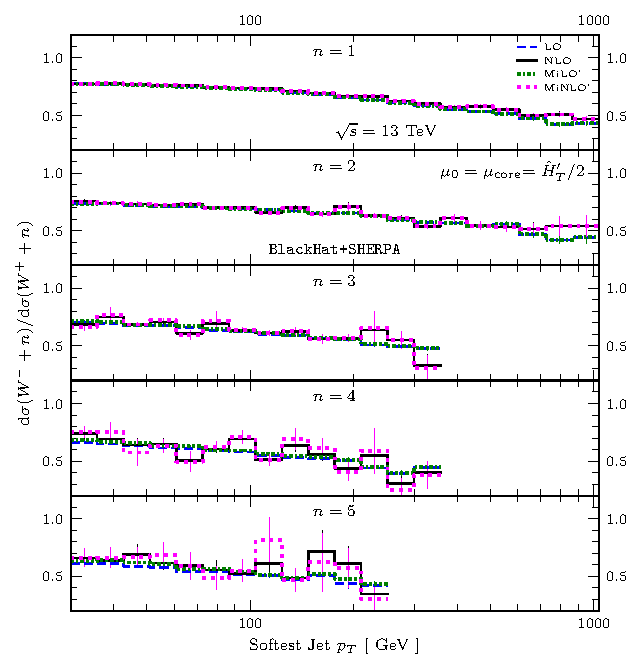
\includegraphics[clip,scale=0.75]{plots/flavorratio_Wm_Wp_13TeV_anti-kt-R4-Pt30_jets_jet_1_1_pt__Kn}
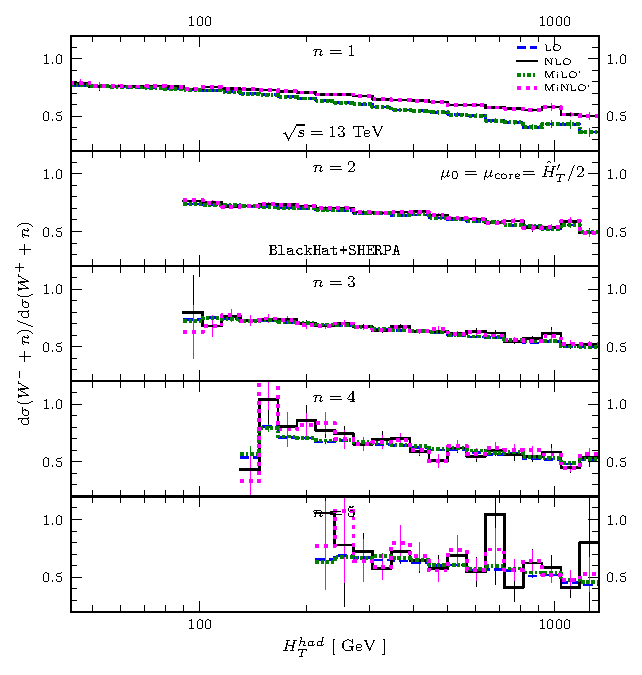
\includegraphics[clip,scale=0.75]{plots/flavorratio_Wm_Wp_13TeV_anti-kt-R4-Pt30_jets_HT_C}
\caption{The charge ratios of \Wmjn-jet to \Wpjn-jet cross sections as a function of
the softest-jet $p_{\textrm T}$ on the left, and as a function of
the hadronic transverse energy $H_{\textrm T}^{had}$ on the right, for results
from $n=2$ (top panel) to $n=5$ (bottom panel). Format as in
Figure~\ref{fig_jetrat}.
}
\label{fig_chargerat}
\end{figure}
%%%%%%%%%%%%%%%%%%%%%%%%%%%%%


In the right panel of Fig.~\ref{fig_jetrat}, we show the differential
ratios in $H_{\textrm T}^{had}$. Similar to the $p_{\textrm T}^W$ ratios, we observe that for $n=2$ the ratio in
$H_{\textrm T}^{had}$ is not stable under the fixed-order quantum
corrections. Even at NLO, the differential jet production ratio is
larger than 1 for a large range of $H_{\textrm T}^{had}$ that is shown. We expect this observable to stabilize if higher-multiplicity results are included either
through NNLO or even higher-order calculations, or through multi-jet
merging at NLO. Around the threshold, all ratios lie at a value of the same order.
With increasing $H_{\textrm T}^{had}$ they increase monotonically and
stabilize at NLO for $n\geq 3$ for large values of
$H_{\textrm T}^{had}$. We observe a characteristic
behavior of the ratios in the high $H_{\textrm T}^{had}$ region. Such events tend to be populated by multiple jets and the $H_{\textrm T}^{had}$
distributions in these jet bins tend to overlap~\cite{BH:Wratios}, which results in
the ratio tending to $1.0$. As for the previous observable,
\MINLOp{} and NLO ratios agree very well, with some discrepancy
between LO and \MILOp{} ratios for the lower-multiplicity cases.


\subsection{Vector-Boson Ratios}
\label{sec_ratiowmwp}
% Z/Wp ratios as function of the softest jets and as function of HT
%%%%%%%%%%%%% FIGURE %%%%%%%%%%%%%%%%%%
\begin{figure}[t]

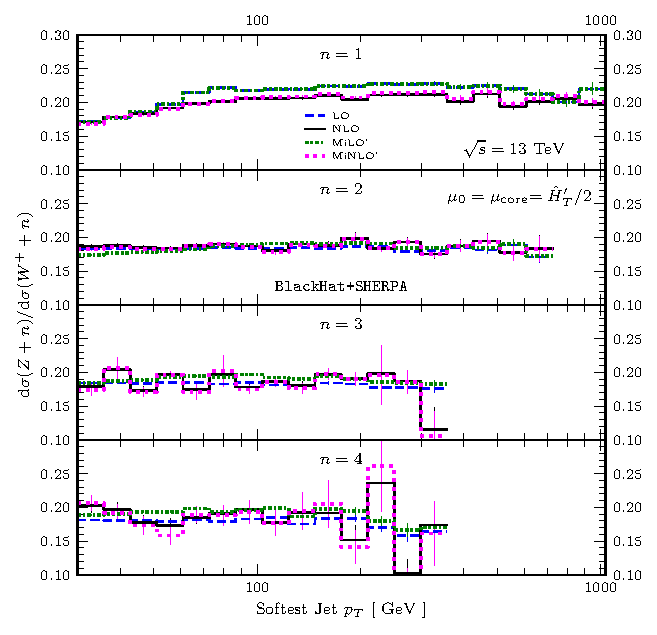
\includegraphics[clip,scale=0.73]{plots/flavorratio_Z_Wp_13TeV_anti-kt-R4-Pt30_jets_jet_1_1_pt__Kn}
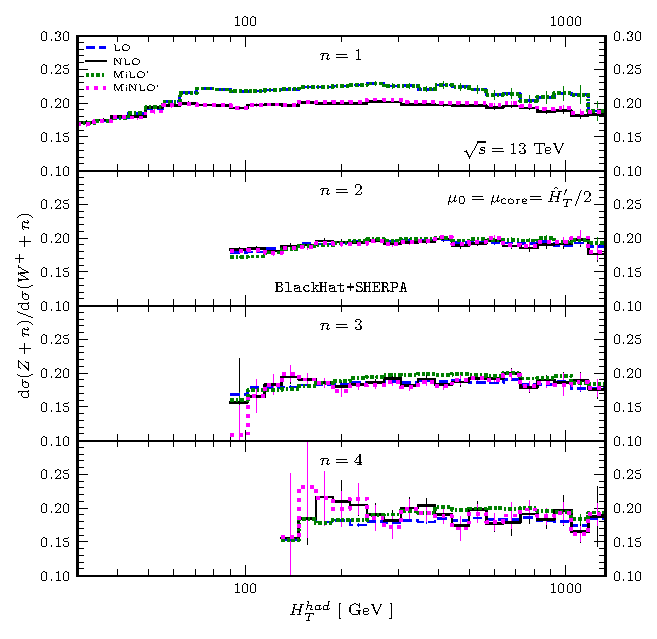
\includegraphics[clip,scale=0.73]{plots/flavorratio_Z_Wp_13TeV_anti-kt-R4-Pt30_jets_HT_C}
\caption{The ratios of \Zjn-jet to \Wpjn-jet cross sections as a function of
the softest-jet $p_{\textrm T}$ on the left, and as a function of
the hadronic transverse energy $H_{\textrm T}^{had}$ on the right. We present
results from $n=1$ (top panel) to $n=4$ (bottom panel). Format as in
Figure~\ref{fig_jetrat}.
}
\label{fig_ZWp_rat}
\end{figure}
%%%%%%%%%%%%%%%%%%%%%%%%%%%%%

In this subsection we show vector-boson ratios of $W^-$ to $W^+$ production as well as
$Z$ to $W^+$ production. These ratios can help in the extraction of valence-quark PDF information for large values
of Bjorken $x$~\cite{BH:Wratios,Kom:2010mv} due to the different coupling of the vector bosons to initial quarks.


We display differential ratios as a function of both the transverse
momentum $p_{\textrm T}$ of the softest jet (left panel) as well as the total hadronic
energy $H_{\textrm T}^{had}$ (right panel) for $W^-$ to $W^+$ production accompanied with
up to five jets in Fig.~\ref{fig_chargerat} and $Z$ to $W^+$ production with up to four jets in Fig.~\ref{fig_ZWp_rat}. We show ratios for both scale choices with
those for $\HTpartonicp/2$ shown at LO as dashed (blue)
lines and at NLO as solid (black) lines, while \MILOp{} ratios are
shown as dash-dotted (green) lines and those for \MINLOp{} as
dotted (magenta) lines. Ratios of $Z$ to $W$ production have been studied experimentally for example
in~\cite{Chatrchyan:2011ne}.


The ratios of $W^-/W^+$ production as a function of the transverse momentum for low values of $p_{\textrm T}$ lie around a value of roughly the same
order for all
shown multiplicities $n$. With increasing $p_{\textrm T}$, we observe a monotonic
decrease of the corresponding ratio. We attribute this decrease to the different couplings of $W^\pm$ bosons to initial quarks, which together with the
dominance of $u$ quarks over $d$ quarks at large values of Bjorken
$x$ leads to a suppression of this ratio. NLO corrections to the transverse momentum ratios are
mild and the results for both scale choices agree very well. We observe a similar behavior for the differential ratios as a function of the total
hadronic energy $H_{\textrm T}^{had}$. In particular, the ratios decrease
monotonically with increasing $H_{\textrm T}^{had}$, 
and take values of the same order at low $H_{\textrm T}^{had}$ for all
multiplicity, also the results for both scale choices agree very
well. However, we observe noticeable NLO correction for the $n=1$ case in
the high $H_{\textrm T}^{had}$ tail.


The ratios of $Z$ to $W^+$ production in Figure~\ref{fig_ZWp_rat} are
quite flat over the full range of variables shown, which is in
contrast to the $W^-/W^+$ ratios in
Figure~\ref{fig_chargerat}. This can be traced to the fact that the Z boson has an appreciable
coupling to initial $u$ quarks, as the $W^+$ boson. The values of $Z/W^+$ ratios as a function
of both the variables shown lie around roughly the same value for all multiplicities $n$ shown. For the $n=1$ case, a slight decrease of the $Z/W^+$ ratio can be observed in the low
$p_{\textrm T}$ region and there are also noticeable quantum corrections in this case. For all the $Z/W^+$
ratios, the results for both scale choices agree very well. In general, the quantum corrections in the $Z/W^+$ observable ratios are
quite mild, which makes them excellent choices for new-physics searches.

